\textbf{📋 Apa yang akan dipelajari}

Pada bab ini kita akan mempelajari tentang Control Statement (Struktur Kendali) dalam C++:

\begin{itemize}
\item Percabangan (if, if-else, switch)
\item Perulangan (for, while, do-while)
\item Kata kunci break dan continue
\end{itemize}

\minitoc

\section{🎯 Pengenalan Control Statement}

Program tidak selalu berjalan secara berurutan dari atas ke bawah. Kadang-kadang kita perlu:
\begin{itemize}
\item \textbf{Percabangan} - memilih jalur program berdasarkan kondisi
\item \textbf{Perulangan} - mengulang perintah tertentu
\item \textbf{Kombinasi} - menggabungkan percabangan dan perulangan
\end{itemize}

Control statement adalah konsep fundamental dalam pemrograman yang memungkinkan program untuk membuat keputusan dan mengulang operasi\footnote{Dijkstra, E. W. (1968). "Go To Statement Considered Harmful". Communications of the ACM.}.

Control Statement adalah pengatur aliran program yang memungkinkan kita:
\begin{itemize}
\item Mengulang perintah jika kondisi tertentu terpenuhi
\item Melanjutkan program jika kondisi terpenuhi
\item Memilih dari beberapa alternatif berdasarkan kondisi
\end{itemize}

\section{🔄 Percabangan (Conditional Statements)}\label{percabangan}

Percabangan adalah perintah yang memungkinkan program memilih jalur yang berbeda berdasarkan kondisi tertentu. 

\subsection{Apa itu Percabangan?}

Percabangan memungkinkan program untuk:
\begin{itemize}
\item Menjalankan kode tertentu jika kondisi terpenuhi
\item Menjalankan kode lain jika kondisi tidak terpenuhi
\item Memilih dari beberapa alternatif berdasarkan nilai tertentu
\end{itemize}

\subsection{Jenis-jenis Percabangan dalam C++}

C++ memiliki tiga jenis perintah percabangan:
\begin{itemize}
\item \textbf{if} - menjalankan kode jika kondisi benar
\item \textbf{if-else} - menjalankan kode berbeda berdasarkan kondisi
\item \textbf{switch} - memilih dari beberapa alternatif berdasarkan nilai
\end{itemize}

\subsection{🔀 Percabangan dengan if}\label{percabangan-dengan-if}

Percabangan \textbf{if} adalah yang paling sederhana. Program akan menjalankan kode di dalam blok if jika kondisi bernilai benar (true). Konsep ini pertama kali diperkenalkan dalam bahasa ALGOL 60\footnote{Naur, P. (1960). "Report on the Algorithmic Language ALGOL 60". Communications of the ACM.}.

\subsubsection{Sintaks if}

\lstinputlisting[language=c++, numbers=none]{../code/control-if-syntax.cpp}

\subsubsection{Cara Kerja if}

\begin{itemize}
\item Program mengecek kondisi dalam kurung
\item Jika kondisi \textbf{benar} (true), kode dalam blok dijalankan
\item Jika kondisi \textbf{salah} (false), kode dalam blok dilewati
\item Program melanjutkan ke baris setelah blok if
\end{itemize}

Flowchart untuk statment percabangan if seperti pada gambar berikut


\begin{tikzpicture}[node distance = 2cm, auto]
\node [ling] (init){start};
\node [decision, below of=init] (decide) {\textless{}ekspresi \_bool\textgreater{}};
\node [block, below of=decide, node distance=3cm] (statement) {Statement};
\node [ling, below of=statement] (stop) {stop};

%garis
\path [line] (init) -- (decide);
\path [line] (init) -- (decide);
\path [line] (decide) -- node {Yes}(statement);
%\path [line] (statement) |- node [near start] {No} (decide);
\path[line] (statement) -- (stop);
\end{tikzpicture}


\subsection*{💡 Contoh Percabangan dengan if}

\begin{enumerate}
\item Buka Qt Creator dan buat project Qt Console Application baru dengan nama "contoh"
\item Tulis kode berikut:

\lstinputlisting[language=c++, caption=Contoh percabangan dengan if, label=contoh2-3]{../code/contoh2-3.cpp}

\item Jalankan program dengan menekan Ctrl + R. Outputnya:

\begin{lcverbatim}
Masukan nomor: 15
15 lebih besar dari 10
\end{lcverbatim}

\subsubsection*{Penjelasan Program}
\begin{itemize}
\item Program meminta input angka dari pengguna
\item Jika angka > 10, program menampilkan pesan "lebih besar dari 10"
\item Jika angka ≤ 10, program tidak menampilkan apa-apa
\end{itemize}
\end{enumerate}
\subsection{🔄 Percabangan dengan if-else}\label{percabangan-dengan-if-..-else}

Percabangan \textbf{if-else} memungkinkan program menjalankan kode yang berbeda berdasarkan kondisi.

\subsubsection{Sintaks if-else}

\lstinputlisting[language=c++]{../code/control-if-else-syntax.cpp}

\subsubsection{Cara Kerja if-else}

\begin{itemize}
\item Program mengecek kondisi dalam kurung
\item Jika kondisi \textbf{benar}, kode dalam blok if dijalankan
\item Jika kondisi \textbf{salah}, kode dalam blok else dijalankan
\item Program selalu menjalankan salah satu blok (if atau else)
\end{itemize}

Flowchart untuk statment ini adalah :

\begin{quotation}
{\LARGE \ding{45}} \textbf{💡 CATATAN PENTING}

Di dalam blok \texttt{if()} maupun \texttt{else} bisa diisi dengan perintah \texttt{if()} lagi. Bentuk \texttt{if()} dalam \texttt{if()} ini sering disebut dengan \textbf{nested if} (if bersarang).
\end{quotation}

\begin{tikzpicture}[node distance = 2cm, auto]
\node [ling] (init){start};
\node [decision, below of=init, node distance=2cm] (decide) {\textless{}ekspresi \_bool\textgreater{}};
\node [block, below of=decide, node distance=3cm] (statement) {Statement};
\node [block, right of=decide, node distance=3cm] (statement2) {Statement2};
\node [ling, below of=statement, node distance=2cm] (stop) {stop};

%garis
\path [line] (init) -- (decide);
\path [line] (init) -- (decide);
\path [line] (decide) -- node {Ya}(statement);
%\path [line] (statement) |- node [near start] {No} (decide);
\path[line] (statement) -- (stop);
\path[line] (statement) -| node {tidak}(statement2);
\path[line] (statement2) -- (decide);
\end{tikzpicture}

\subsubsection*{💡 Contoh Program if-else}

\begin{enumerate}
\item Edit contoh \ref{contoh2-3} dengan menambahkan kode berikut:

\lstinputlisting[language=c++, firstline=13, lastline=14, caption=Contoh percabangan if-else, label=contoh2-4]{../code/contoh2-4.cpp}

\item Jalankan program dengan menekan Ctrl + R. Outputnya:

\begin{lcverbatim}
Masukan nomor: 4
4 kurang besar dari 10
\end{lcverbatim}

\subsubsection*{Penjelasan Program}
\begin{itemize}
\item Jika angka > 10, program menampilkan "lebih besar dari 10"
\item Jika angka ≤ 10, program menampilkan "kurang besar dari 10"
\item Program selalu memberikan respons, tidak ada kondisi yang dilewati
\end{itemize}
\end{enumerate}

\subsection{🔄 Percabangan dengan if Bersarang (Nested if)}

If bersarang adalah kondisi if yang berada di dalam blok if atau else lainnya. Ini memungkinkan kita membuat percabangan yang lebih kompleks.

\subsubsection{Cara Kerja Nested if}

\begin{itemize}
\item Program mengecek kondisi if pertama
\item Jika benar, program mengecek kondisi if kedua
\item Jika salah, program bisa mengecek kondisi if lain atau menjalankan else
\item Bisa dibuat bertingkat sesuai kebutuhan
\end{itemize}

Flowchart untuk statement if bersarang:

\begin{tikzpicture}[node distance = 1cm, auto]
\node [ling] (init){start};
\node [decision, below of=init, node distance=3cm] (decide) {\textless{}ekspresi \_bool\textgreater{}};
\node [block, below of=decide, node distance=3cm] (statement) {Statement};

\node [decision, right of=decide, node distance=3cm] (decide1) {\textless{}ekspresi \_bool\textgreater{}};
\node [block, below of=decide1, node distance=3cm] (statement1) {Statement1};

\node [block, right of=decide1, node distance=6cm] (statement2) {Statement2};
\node [ling, below of=statement, node distance=2cm] (stop) {stop};

%garis
\path [line] (init) -- (decide);
\path [line] (decide) -- node{Tidak}(decide1);
\path [line,dashed](decide1) -- node{tidak\dots dst \dots tidak }(statement2);
\path [line] (decide) -- node{Ya}(statement);
\path [line] (decide1) -- node {Ya} (statement1);
\path[line] (statement) -- (stop);

\path[line] (statement2) |- (stop);
\path[line] (statement1) |- (stop);
\path [line] (decide) -- node {Ya}(statement);

\end{tikzpicture}

\subsection{🔀 Percabangan dengan switch}\label{percabangan-dengan-switch}

Percabangan \textbf{switch} digunakan sebagai alternatif dari \texttt{if-else} ketika kita memiliki banyak pilihan berdasarkan nilai tertentu. Switch statement diperkenalkan dalam bahasa C dan kemudian diadopsi oleh C++\footnote{Kernighan, B. W., \& Ritchie, D. M. (1988). "The C Programming Language" (2nd ed.). Prentice Hall.}.

\subsubsection{Kapan Menggunakan switch}

\begin{itemize}
\item Ketika ada banyak pilihan berdasarkan nilai yang sama
\item Lebih efisien daripada if-else bertingkat
\item Hanya bisa membandingkan nilai yang sama (==), bukan operator pembanding (<, >, dll)
\item Ekspresi harus menghasilkan nilai bulat (int, char, enum)
\end{itemize}

\subsubsection{Keuntungan switch}

\begin{itemize}
\item Lebih mudah dibaca untuk banyak pilihan
\item Lebih efisien dalam eksekusi
\item Struktur yang lebih rapi
\end{itemize}

\subsubsection{Sintaks switch}

\lstinputlisting[language=c++, numbers=none]{../code/control-switch-syntax.cpp}

\subsubsection{Cara Kerja switch}

\begin{enumerate}
\item Program mengevaluasi \textbf{ekspresi} dalam switch
\item Membandingkan hasil dengan nilai di setiap \textbf{case}
\item Jika ada yang cocok, menjalankan pernyataan di case tersebut
\item \textbf{break} menghentikan eksekusi switch
\item Jika tidak ada yang cocok, menjalankan \textbf{default}
\end{enumerate}

\subsubsection{Pentingnya break}

\begin{itemize}
\item \textbf{break} menghentikan eksekusi switch
\item Tanpa break, program akan melanjutkan ke case berikutnya
\item Ini bisa menyebabkan eksekusi yang tidak diinginkan
\end{itemize}

Flowchart untuk statement ini adalah :

\begin{tikzpicture}[node distance = 1cm, auto]
\node [blok] (ekspresi) {\textless{}nilai\_ekspresi1\textgreater{}};
\node [blok,below of=ekspresi] (ekspresi1) {\textless{}nilai\_ekspresi2\textgreater{}};
\node [blok,below of=ekspresi1] (ekspresi2) {\textless{}nilai\_ekspresi3\textgreater{}};
\node [blok,below of=ekspresi2] (ekspresi3) {\textless{}nilai\_ekspresi4\textgreater{}};
\node [blok,below of=ekspresi3, node distance=2cm] (ekspresi4) {\textless{}nilai\_lainya\textgreater{}};

\node [titik, left of=ekspresi2, node distance=2cm] (titik) {};
\node [decision, left of=titik, node distance=2cm] (decide) {\textless{}ekspresi\textgreater{}};

\node [blok, right of=ekspresi, node distance=4cm] (statement) {\textless{}statement1\textgreater{}};
\node [blok,below of=statement] (statement1) {\textless{}statement2\textgreater{}};
\node [blok,below of=statement1] (statement2) {\textless{}statement3\textgreater{}};
\node [blok,below of=statement2] (statement3) {\textless{}statement4\textgreater{}};
\node [blok,below of=statement3, node distance=2cm] (statement4) {\textless{}statement\textgreater{}};

\node [ling, above of=decide, node distance=3cm] (start) {start};
\node [ling, right of=statement4, node distance=3cm] (stop) {stop};


\path[line](start) -- (decide);
\path[line](titik) |- (ekspresi);
\path[line](titik) |- (ekspresi1);
\path[line](titik) |- (ekspresi2);
\path[line](titik) |- (ekspresi3);
\path[line](titik) |- (ekspresi4);
\path[line,dashed](ekspresi3) -- node{dst}(ekspresi4);

\path[line](ekspresi) -- (statement);
\path[line](ekspresi1) -- (statement1);
\path[line](ekspresi2) -- (statement2);
\path[line](ekspresi3) -- (statement3);
\path[line](ekspresi4) -- (statement4);
\path[line,dashed](statement3) -- node{dst}(statement4);

\path[line](statement) -| (stop);
\path[line](statement1) -| (stop);
\path[line](statement2) -| (stop);
\path[line](statement3) -| (stop);
\path[line](statement4) -- (stop);

\path[line](decide) -- (titik);
\end{tikzpicture}



\subsection{💡 Contoh Program switch}

\begin{enumerate}
\item Buka Qt Creator dan buat project Qt Console Application baru dengan nama "contoh"
\item Tulis kode berikut:

\lstinputlisting[language=c++, caption=Contoh program switch, label=contoh2-2]{../code/contoh2-2.cpp}

\item Jalankan program dengan menekan Ctrl + R. Outputnya:

\begin{lcverbatim}
sabtu
\end{lcverbatim}
\end{enumerate}

\subsubsection*{Penjelasan Program}

\begin{itemize}
\item Variabel \texttt{hari} dideklarasikan bertipe \texttt{int} dengan nilai \texttt{6}
\item Program mengevaluasi nilai \texttt{hari} dalam switch
\item Karena nilai = 6, program menjalankan \texttt{case 6}
\item Program menampilkan "sabtu" ke layar
\end{itemize}

\section{🔄 Perulangan (Loops)}\label{perulangan}

Perulangan digunakan untuk mengulang suatu perintah sebanyak yang diinginkan tanpa harus menulis ulang kode yang sama.

\subsection{Apa itu Perulangan?}

Perulangan memungkinkan program untuk:
\begin{itemize}
\item Mengulang kode tertentu berkali-kali
\item Menjalankan kode sampai kondisi tertentu terpenuhi
\item Menghemat penulisan kode yang berulang
\end{itemize}

\subsection{Jenis-jenis Perulangan dalam C++}

C++ memiliki tiga jenis perintah perulangan:
\begin{itemize}
\item \textbf{for} - perulangan dengan jumlah yang diketahui
\item \textbf{while} - perulangan selama kondisi benar
\item \textbf{do-while} - perulangan yang minimal dijalankan sekali
\end{itemize}

\subsection{🔄 Perulangan dengan for}\label{perulangan-dengan-for}

Perulangan \textbf{for} digunakan ketika kita sudah mengetahui berapa kali perulangan akan dijalankan. For loop adalah salah satu konstruksi perulangan yang paling umum digunakan dalam pemrograman\footnote{Knuth, D. E. (1997). "The Art of Computer Programming, Volume 1: Fundamental Algorithms" (3rd ed.). Addison-Wesley.}.

\subsubsection{Kapan Menggunakan for}

\begin{itemize}
\item Jumlah perulangan sudah diketahui
\item Perulangan dengan counter yang teratur
\item Iterasi melalui array atau range tertentu
\end{itemize}

\subsubsection{Sintaks for}

\lstinputlisting[language=c++, numbers=none]{../code/control-for-syntax.cpp}

\subsubsection{Komponen for}

\begin{itemize}
\item \textbf{nilai\_awal} - inisialisasi variabel counter
\item \textbf{kondisi} - syarat untuk melanjutkan perulangan
\item \textbf{perubahan} - cara mengubah nilai counter (biasanya increment/decrement)
\end{itemize}

\begin{figure}[htbp]
\centering
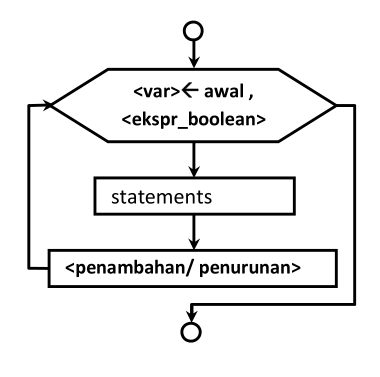
\includegraphics[width=8cm]{Capture2-8}
\caption{flowchart perulangan dengan for}
\end{figure}

\subsection{🔄 Perulangan dengan while}\label{perulangan-dengan-while}

Perulangan \textbf{while} digunakan untuk mengulangi perintah selama kondisi masih bernilai benar.

\subsubsection{Kapan Menggunakan while}

\begin{itemize}
\item Jumlah perulangan tidak diketahui
\item Perulangan berdasarkan kondisi tertentu
\item Perulangan yang berhenti ketika kondisi menjadi salah
\end{itemize}

\subsubsection{Sintaks while}

\lstinputlisting[language=c++, numbers=none]{../code/control-while-syntax.cpp}

\subsubsection{Cara Kerja while}

\begin{itemize}
\item Program mengecek kondisi sebelum masuk perulangan
\item Jika kondisi benar, kode dalam blok dijalankan
\item Setelah kode selesai, kondisi dicek lagi
\item Perulangan berhenti ketika kondisi menjadi salah
\end{itemize}

\begin{figure}[htbp]
\centering
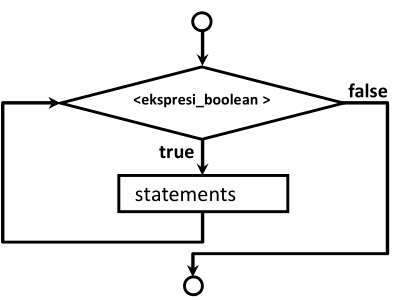
\includegraphics[width=8cm]{Capture2-9}
\caption{flowchart perulangan dengan while}
\end{figure}

\subsection{🔄 Perulangan dengan do-while}\label{perulangan-dengan-do-while}

Perulangan \textbf{do-while} mirip dengan while, tetapi kondisi dicek di akhir perulangan. Ini berarti kode minimal akan dijalankan sekali.

\subsubsection{Kapan Menggunakan do-while}

\begin{itemize}
\item Ketika kode minimal harus dijalankan sekali
\item Perulangan yang kondisi pengecekannya di akhir
\item Menu atau input yang perlu diproses minimal sekali
\end{itemize}

\subsubsection{Sintaks do-while}

\lstinputlisting[language=c++, numbers=none]{../code/control-do-while-syntax.cpp}

\subsubsection{Cara Kerja do-while}

\begin{itemize}
\item Program menjalankan kode dalam blok do terlebih dahulu
\item Setelah kode selesai, kondisi dicek
\item Jika kondisi benar, perulangan dilanjutkan
\item Jika kondisi salah, perulangan berhenti
\end{itemize}

\begin{figure}[htbp]
\centering
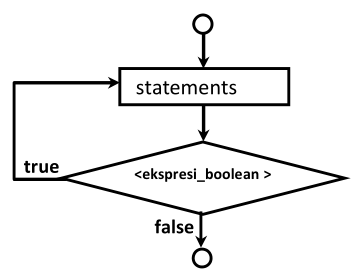
\includegraphics[width=8cm]{Capture2-10}
\caption{flowchart perulangan dengan do\dots while}
\end{figure}

\subsection{📊 Perbandingan while vs do-while}

\begin{center}
\begin{tabular}{|l|l|l|}
\hline
\textbf{Aspek} & \textbf{while} & \textbf{do-while} \\
\hline
Pengecekan kondisi & Di awal & Di akhir \\
\hline
Minimal eksekusi & 0 kali & 1 kali \\
\hline
Kapan digunakan & Kondisi mungkin salah di awal & Kode harus dijalankan minimal sekali \\
\hline
\end{tabular}
\end{center}

\subsubsection{Perbedaan Utama}

\begin{itemize}
\item \textbf{while}: kondisi dicek sebelum masuk perulangan
\item \textbf{do-while}: kondisi dicek setelah menjalankan kode
\item \textbf{while}: mungkin tidak menjalankan kode sama sekali
\item \textbf{do-while}: minimal menjalankan kode sekali
\end{itemize}

\subsection{⏭️ Kata Kunci break dan continue}\label{kata-kunci-continue-dan-break}

Kata kunci \textbf{break} dan \textbf{continue} digunakan untuk mengontrol aliran perulangan.

\subsubsection{Kata Kunci break}

\begin{itemize}
\item \textbf{break} menghentikan perulangan secara total
\item Program keluar dari perulangan dan melanjutkan ke baris setelah perulangan
\item Bisa digunakan dalam for, while, do-while, dan switch
\end{itemize}

\subsubsection{Kata Kunci continue}

\begin{itemize}
\item \textbf{continue} melompati iterasi saat ini
\item Program melanjutkan ke iterasi berikutnya
\item Kode setelah continue dalam iterasi yang sama tidak dijalankan
\end{itemize}

\subsubsection{Sintaks break dan continue}

\lstinputlisting[language=c++]{../code/02-control-statement-code-1.c++}

\subsection{💡 Contoh Program break dan continue}

\begin{enumerate}
\item Buka Qt Creator dan buat project Qt Console Application baru dengan nama "contoh"
\item Tulis kode berikut:

\lstinputlisting[language=c++, caption=Contoh penggunaan break dan continue, label=contoh2-5]{../code/contoh2-5.cpp}

\item Jalankan program dengan menekan Ctrl + R. Outputnya:

\begin{lcverbatim}
1 2 3 4 6 7 8 9 10
Loop berhenti karena break
\end{lcverbatim}
\end{enumerate}

\subsubsection*{Penjelasan Program}
\begin{itemize}
\item Program menggunakan perulangan for dari 1 sampai 10
\item Jika i == 5, program menggunakan continue untuk melompati angka 5
\item Jika i == 10, program menggunakan break untuk menghentikan perulangan
\item Hasilnya: angka 1-4, 6-9 ditampilkan, lalu loop berhenti
\end{itemize}

\section{🎯 Praktik Terbaik Control Statement}

\subsection{💡 Tips Menulis Control Statement yang Baik}

\begin{enumerate}
\item \textbf{Gunakan kondisi yang jelas} - Hindari kondisi yang membingungkan
\item \textbf{Tulis kode yang mudah dibaca} - Gunakan indentasi yang konsisten
\item \textbf{Hindari nested if yang terlalu dalam} - Maksimal 3-4 tingkat
\item \textbf{Gunakan switch untuk banyak pilihan} - Lebih efisien daripada if-else bertingkat
\item \textbf{Selalu gunakan kurung kurawal} - Meskipun hanya satu baris kode
\end{enumerate}

\subsection{⚠️ Kesalahan Umum yang Harus Dihindari}

\begin{itemize}
\item \textbf{Lupa break dalam switch} - Bisa menyebabkan fall-through
\item \textbf{Infinite loop} - Perulangan yang tidak pernah berhenti
\item \textbf{Kondisi yang selalu benar/salah} - Perulangan atau percabangan yang tidak efektif
\item \textbf{Indentasi yang salah} - Membuat kode sulit dibaca
\end{itemize}

\section{📊 Ringkasan Control Statement}

\subsection{🔄 Jenis-jenis Control Statement}

\begin{center}
\begin{tabular}{|l|l|l|}
\hline
\textbf{Jenis} & \textbf{Kegunaan} & \textbf{Contoh} \\
\hline
if & Percabangan sederhana & if (x > 0) \\
\hline
if-else & Percabangan dengan alternatif & if (x > 0) else \\
\hline
switch & Banyak pilihan & switch (x) case 1: \\
\hline
for & Perulangan dengan counter & for (int i=0; i<n; i++) \\
\hline
while & Perulangan dengan kondisi & while (x > 0) \\
\hline
do-while & Perulangan minimal sekali & do \{ \} while (x > 0) \\
\hline
break & Menghentikan perulangan & break; \\
\hline
continue & Melompati iterasi & continue; \\
\hline
\end{tabular}
\end{center}

\subsection{🎯 Kapan Menggunakan Setiap Jenis}

\begin{itemize}
\item \textbf{if}: Ketika ada satu kondisi yang perlu dicek
\item \textbf{if-else}: Ketika ada dua alternatif yang berbeda
\item \textbf{switch}: Ketika ada banyak pilihan berdasarkan nilai yang sama
\item \textbf{for}: Ketika jumlah perulangan sudah diketahui
\item \textbf{while}: Ketika jumlah perulangan tidak diketahui
\item \textbf{do-while}: Ketika kode minimal harus dijalankan sekali
\item \textbf{break}: Ketika perlu menghentikan perulangan secara paksa
\item \textbf{continue}: Ketika perlu melompati iterasi tertentu
\end{itemize}

\section{🔍 Latihan dan Soal}

\subsection{📝 Latihan 1: Program Kalkulator Sederhana}

Buat program kalkulator sederhana yang menerima dua angka dan operator (+, -, *, /) dari pengguna, kemudian menampilkan hasilnya.

\subsection{📝 Latihan 2: Program Menentukan Grade}

Buat program yang menerima nilai (0-100) dan menampilkan grade:
\begin{itemize}
\item A: 90-100
\item B: 80-89
\item C: 70-79
\item D: 60-69
\item E: 0-59
\end{itemize}

\subsection{📝 Latihan 3: Program Menampilkan Pola}

Buat program yang menampilkan pola bintang seperti berikut:
\begin{lcverbatim}
*
**
***
****
*****
\end{lcverbatim}

\section{📚 Referensi dan Bacaan Lanjutan}

Control statement adalah konsep fundamental dalam pemrograman yang telah dikembangkan sejak awal era komputer. Konsep ini pertama kali diperkenalkan dalam bahasa pemrograman FORTRAN pada tahun 1957\footnote{Backus, J. W. (1957). "The FORTRAN Automatic Coding System". Proceedings of the Western Joint Computer Conference.} dan kemudian dikembangkan lebih lanjut dalam bahasa ALGOL\footnote{Naur, P. (1960). "Report on the Algorithmic Language ALGOL 60". Communications of the ACM.}.

Dalam konteks C++, control statement mengikuti tradisi bahasa C yang dikembangkan oleh Dennis Ritchie di Bell Labs pada tahun 1972\footnote{Ritchie, D. M. (1993). "The Development of the C Language". ACM SIGPLAN Notices.}. Bjarne Stroustrup kemudian mengembangkan C++ dengan menambahkan fitur object-oriented programming sambil mempertahankan sintaks control statement yang familiar\footnote{Stroustrup, B. (1994). "The Design and Evolution of C++". Addison-Wesley.}.

Untuk pemahaman yang lebih mendalam tentang control statement dalam C++, pembaca dapat merujuk pada:

\begin{itemize}
\item \textbf{The C++ Programming Language} oleh Bjarne Stroustrup\footnote{Stroustrup, B. (2013). "The C++ Programming Language" (4th ed.). Addison-Wesley.}
\item \textbf{Effective C++} oleh Scott Meyers\footnote{Meyers, S. (2005). "Effective C++" (3rd ed.). Addison-Wesley.}
\item \textbf{C++ Primer} oleh Stanley Lippman\footnote{Lippman, S. B., Lajoie, J., \& Moo, B. E. (2012). "C++ Primer" (5th ed.). Addison-Wesley.}
\end{itemize}

\section{🎉 Kesimpulan}

Control statement adalah alat fundamental yang memungkinkan program untuk membuat keputusan dan mengulang operasi. Dengan menguasai konsep ini, Anda telah memiliki fondasi yang kuat untuk mengembangkan program yang lebih kompleks dan dinamis.

\begin{center}
\textbf{Selamat! Anda telah menguasai dasar-dasar Control Statement dalam C++} 🎯
\end{center}

\vspace{1cm}

\begin{center}
\textit{--- Bab selanjutnya: Array dan String ---}
\end{center}